\documentclass[12pt,letterpaper]{report}

\usepackage[intlimits]{amsmath}
\usepackage[utf8]{inputenc}
\DeclareUnicodeCharacter{2212}{-}
\usepackage{amsfonts,amssymb}
\DeclareSymbolFontAlphabet{\mathbb}{AMSb}
\usepackage{textcomp}

\usepackage{float}
\usepackage[]{caption,subcaption}
\setcaptionmargin{0.5in}

\usepackage{ifthen}
\usepackage{lscape,afterpage}
\usepackage{xspace}
\usepackage{siunitx}
\usepackage{xcolor}

\usepackage{appendix}

\usepackage{enumitem}
\usepackage{graphicx}

\usepackage[htt]{hyphenat}

\newcommand{\figref}[1]{Figure~\ref{#1}}
\newcommand{\mus}[1]{\SI{#1}{\micro s}\xspace}
\def\gmtwo{$g-2$\xspace}
\def\wa{$\omega_{a}$\xspace}


\graphicspath{{Figures/}}


\begin{document}

\section*{Problems with the Vertical Waist in the Ratio Method Analysis}


The necessary inclusion of the VW in the Ratio Method analysis is not immediately apparent, as shown by \figref{fig:FFT_3param_allTimes}. (Incidentally this is also true for the CBO and other effects.) Compared to the FFT of the fit residuals of a five parameter function fit to the data, no peaks rise significantly above the noise. When looking at the FFT of the fit residuals for early times however, as in \figref{fig:FFT_3param_earlyTimes}, a small VW peak can be seen. (As well as the larger CBO peak.) It should be noted here that this small VW peak does not appear for every random seed. The time randomization of the data means that sometimes this VW peak is indistinguishable within the noise. 


\begin{figure}[]
    \centering
    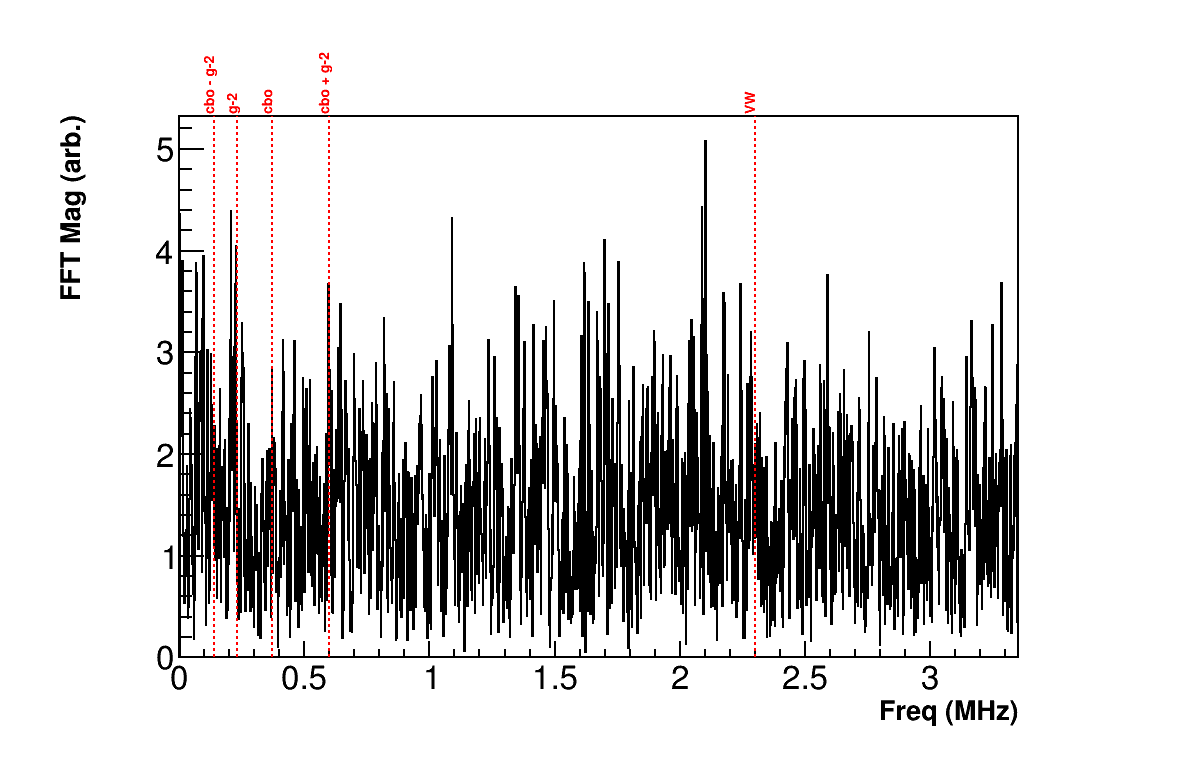
\includegraphics[width=\textwidth]{FFT_3param_allTimes}
    \caption[]{FFT of fit residuals using a 3 parameter ratio function to fit the 60h dataset. The FFT is over all times, \SIrange{30.2}{650}{\micro s}. From file \texttt{/gm2/data/users/nkinnaird/Ratio/60h-FinalProduction/RandSeeds/FitIterations/output-60h-FinalProduction-RandSeeds-1sttest.root} \texttt{FitPass0}.}
    \label{fig:FFT_3param_allTimes}
\end{figure}

\begin{figure}[]
    \centering
    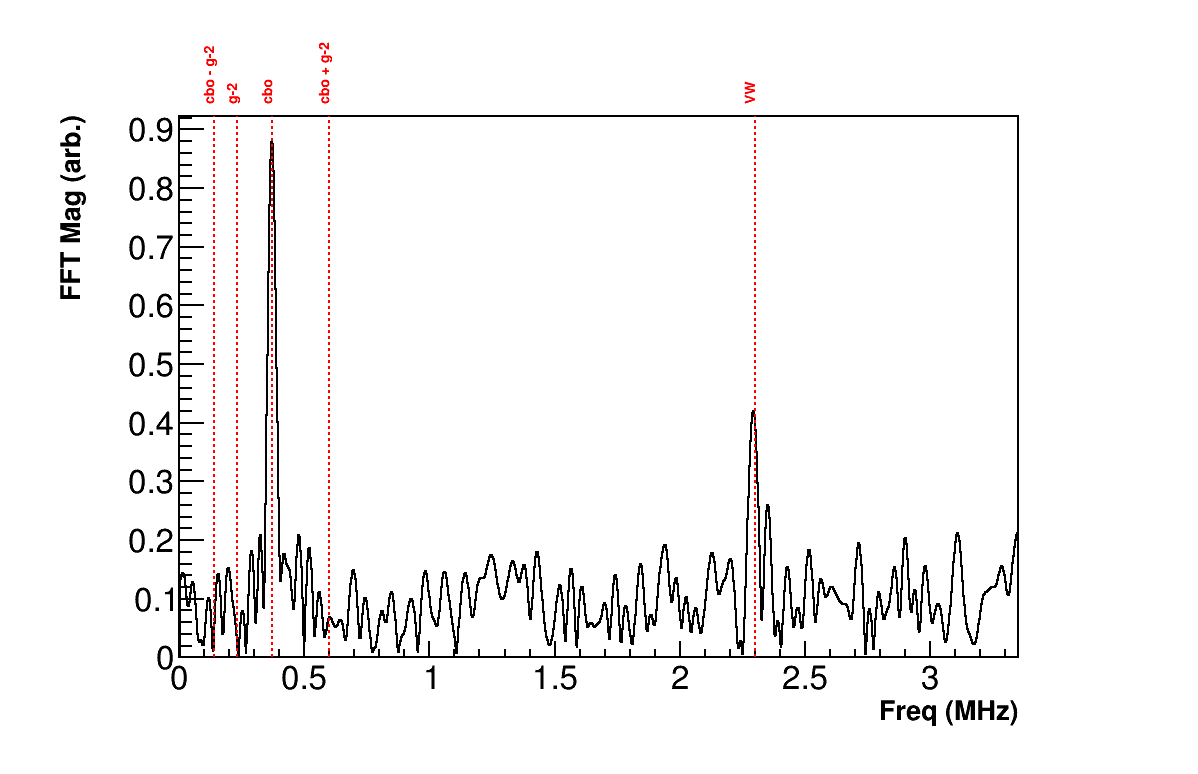
\includegraphics[width=\textwidth]{FFT_3param_earlyTimes}
    \caption[]{FFT of fit residuals using a 3 parameter ratio function to fit the 60h dataset. The FFT is over early times, \SIrange{30.2}{60.2}{\micro s}. From file \texttt{/gm2/data/users/nkinnaird/Ratio/60h-FinalProduction/RandSeeds/FitIterations/output-60h-FinalProduction-RandSeeds-1sttest.root} \texttt{FitPass0}.}
    \label{fig:FFT_3param_earlyTimes}
\end{figure}


The smallness of the VW signal in the ratio method analysis is the first of the problems in including it in the fit. First one might ask however whether it should be included in the fit at all. There are a couple of reasons why I think it should probably be included:
\begin{enumerate}
	\item\label{item:FFTpeak}{A peak in the FFT of the fit residuals can be seen.}
	\item\label{item:VWamp}{When the amplitude of the VW is allowed to float (with some or all of the others parameters fixed, whatever configuration is necessary to get a converging fit), then the VW amplitude converges to a non-zero value.}
	\item\label{item:pVal}{The p value of the fit improves when including the VW, on the order of 8\% for the 60h dataset, and on the order of 40\% for the Endgame dataset. This is reflected in a fit start scan of the p value, which shows a rise for the first \SIrange{20}{30}{\micro s} of the fit or so.}
	\item\label{item:Rchange}{The value of R changes on the order of \SIrange{30}{60}{ppb} depending on the dataset, which parameters are fixed, and what the random seed is.}
\end{enumerate}
It is the combination of items \ref{item:FFTpeak} and \ref{item:pVal} that I think are the real suggestions that I should be including the VW in the ratio fits. A couple of confusing things end up arising though, both around the idea that I should need to include the VW and what I see when I do so.


\subsection*{60h and Endgame Datasets}

The 60h and Endgame datasets run at an n value of 0.108, which just so happens to put the VW frequency at nearly 10 times the \gmtwo frequency, specifically $\omega_{VW} \approx 10.04 \cdot \omega_{a}$ at $t = \infty$. (Remember that in these datasets the CBO frequency and by extension the VW frequency is changing over time, making this whole picture more complicated.) The ratio method, by definition, extracts out the \gmtwo frequency and by extension divides out frequencies which are an even multiple of the \gmtwo frequency. This can be seen in \figref{fig:VW1x-10x}, and the same is shown in a different way in \figref{fig:VWRatioDiff}.


\begin{figure}[]
    \centering
    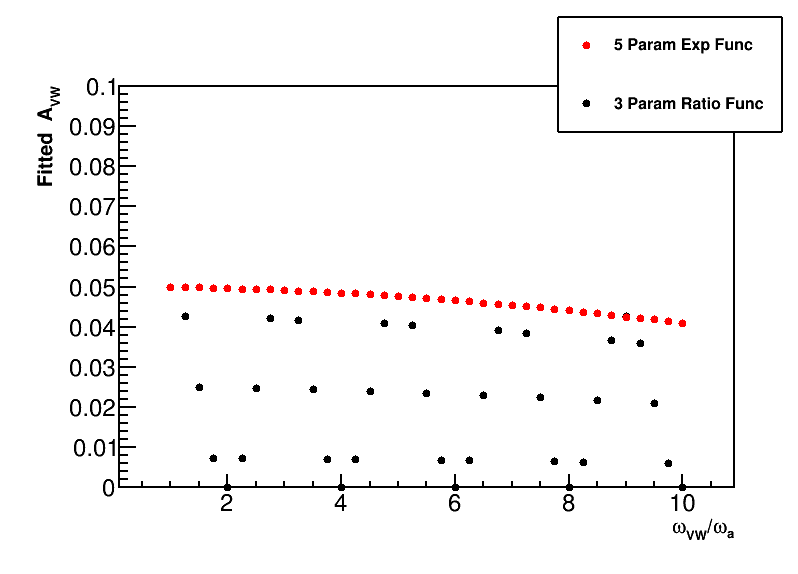
\includegraphics[width=\textwidth]{Fitted_Avw_Vs_Wvw_1x-10x}
    \caption[]{Fitted VW amplitude in a Toy MC as a function of the VW frequency divided by the \gmtwo frequency. In red are the fitted amplitdues with a simple five parameter function, and in black are the fitted amplitudes with a three parameter ratio function. The input VW amplitude was 0.05, and the VW effect was constant throughout the Toy MC "fill." There is a slight fall off of the red points due to the effects of the higher frequencies interacting with the bin width causing a reduction in the fitted amplitude; if an integral fit is used then this fall off is eliminated. What can be seen is that for even frequencies the VW effect dies away, while for odd frequencies it does not. It should be noted here that it doesn't matter that the VW effect is a "high frequency effect,", simply that it is at an even multiple of \wa.}
    \label{fig:VW1x-10x}
\end{figure}



\begin{figure}[]
    \centering
    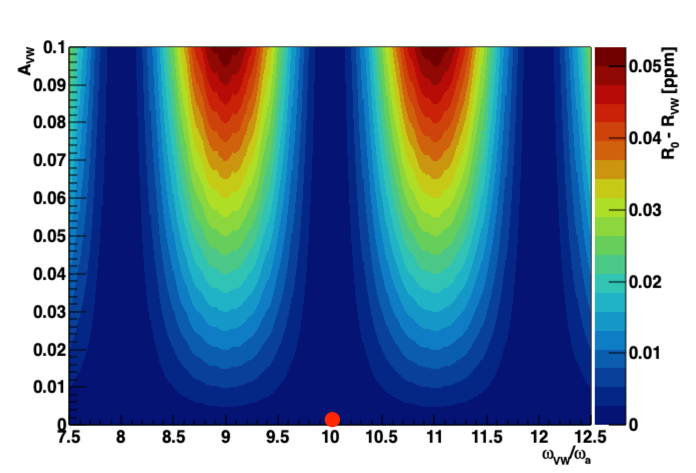
\includegraphics[width=\textwidth]{VWRatioDiff}
    \caption[]{Plotted is the difference in the maximum value of the ratio with and without a VW function included, as a function of both the amplitude of the VW effect and the VW frequency in units of the \gmtwo frequency, in a toy Monte-Carlo simulation. Note that this is not $\boldsymbol{R}$ the frequency fit parameter, but the actual value of the ratio fit function. The difference reaches a minimum for even multiples of the \gmtwo frequency, where the VW effect divides out almost entirely. The $n = 0.108$ datasets, including the 60h and Endgame datasets, live at the bottom center of this plot, marked by a red circle, where the VW frequency is nearly equal to 10 times the \gmtwo frequency, and the difference in the ratio is approximately \SI{5e-6}{} at 30 $\mu s$. Plot courtesy of James Mott.}
    \label{fig:VWRatioDiff}
\end{figure}


\begin{figure}[]
\centering
    \begin{subfigure}[]{0.46\textwidth}
        \centering
        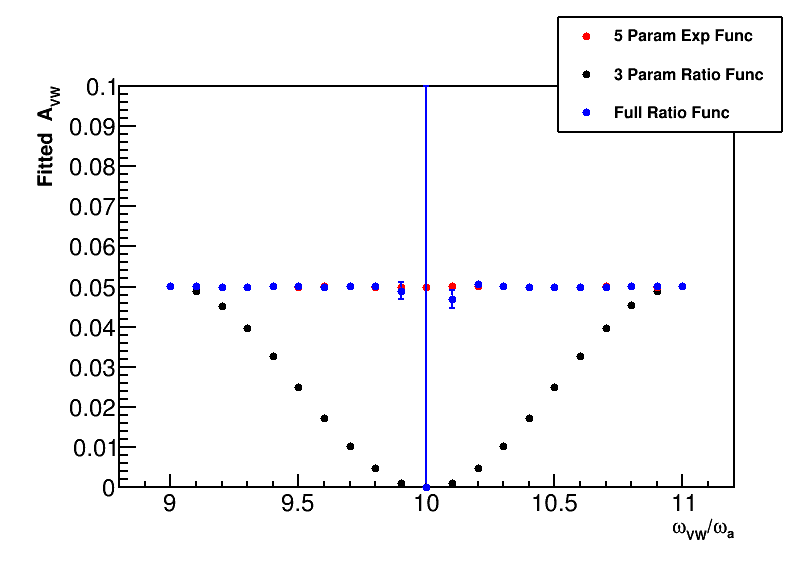
\includegraphics[width=\textwidth]{Fitted_Avw_Vs_Wvw-9x-10x}
        \caption{}
    \end{subfigure}% %you need this % here to add spacing between subfigures
    \hspace{1cm}
    \begin{subfigure}[]{0.46\textwidth}
        \centering
        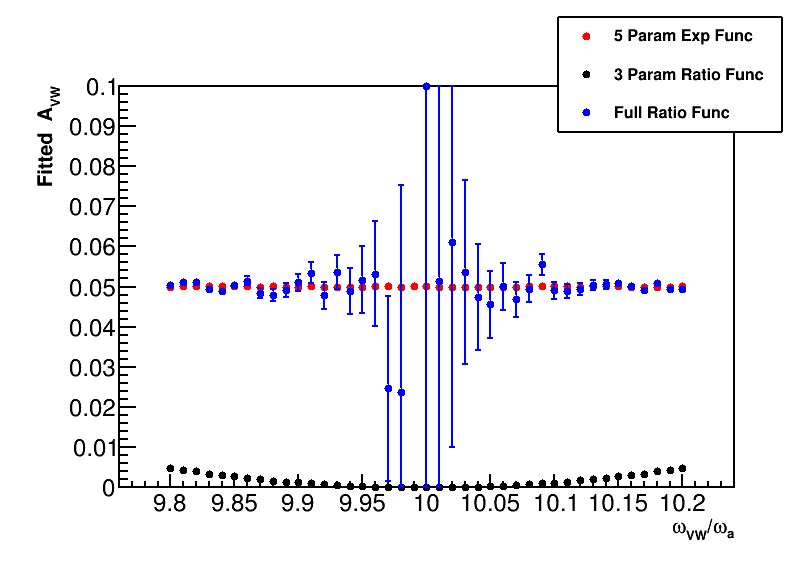
\includegraphics[width=\textwidth]{Fitted_Avw_Vs_Wvw-10x}
        \caption{}
    \end{subfigure}
\caption[]{\textbf{update pictures as needed}}
\label{fig:}
\end{figure}


So the first question is posed as to why ... 





\subsection*{9d Dataset}



\subsection*{Correlations and fit start scans}





-even frequency multiple
-changing frequency though
-reduction in signal
-possibly improper fit function

-contradictions


-unstable fit start scans and correlations


9d
-reduced amplitude in ratio method compared to t method


-keep in mind which parameters are fixed and which are not in the various fits and fit start time scans



worries:
-am I fitting the noise in some way
-am I fitting some other effect
-have I implemented the VW wrongly




methods of trying to solve it:
-either fix it
-figure out what I need to do
-understand mathematically what is going on
-reproduce it in Toy MC and just say it's okay








-what I see
-what the problems are
-what I think
-what I expect
-what's confusing
-what I've tried








% \begin{figure}[]
%     \centering
%     \includegraphics[width=\textwidth]{}
%     \caption[]{}
%     \label{fig:}
% \end{figure}


\end{document}
